\documentclass[aspectratio=169]{beamer}

% Bibliography (if needed)
\usepackage[backend=biber,style=apa]{biblatex}
\addbibresource{refs.bib}

% Math and Graphics
\usepackage{amsmath}
\usepackage{graphicx}
\usepackage{tikz}
\usetheme{metropolis}

% Title Info
\title{Nepali Sentiment Analysis of Post-COVID Data}
\subtitle{Using XLMRoberta for Text Classification}
\author{Amulya Bhandari \and Sailesh Dahal \and Sarayu Gautam \and Tohfa Niraula}
\institute{Department of Computer Engineering\\Kathmandu University}
\date{\today}

\begin{document}

% Title Slide
\maketitle

% Outline
\begin{frame}{Outline}
  \tableofcontents
\end{frame}

% Introduction
\section{Introduction}
\begin{frame}{What is Sentiment Analysis?}
  \begin{itemize}
    \item Sentiment analysis classifies text based on emotion or opinion.
    \item Categories:
          \begin{itemize}
            \item Positive — praise, approval
            \item Neutral — factual
            \item Negative — criticism, disapproval
          \end{itemize}
    \item Applications:
          \begin{itemize}
            \item Social media monitoring
            \item Product reviews
            \item Survey analysis
          \end{itemize}
  \end{itemize}
\end{frame}

% Problem Statement
\section{Problem Statement}
\begin{frame}{What Are We Solving?}
  \begin{itemize}
    \item Goal: Classify Nepali-language text into sentiment categories.
    \item Motivation:
          \begin{itemize}
            \item Nepali is underrepresented in NLP.
            \item Lack of labeled Nepali datasets.
          \end{itemize}
    \item Objectives:
          \begin{enumerate}
            \item Clean and preprocess post-COVID Nepali data.
            \item Train a multilingual BERT model.
            \item Evaluate performance using real-world test data.
          \end{enumerate}
  \end{itemize}
\end{frame}

% Dataset Description
\section{Dataset Description}
\begin{frame}{About the Dataset}
  \begin{itemize}
    \item Source: Nepali COVID/post-COVID text samples.
    \item Total Samples:
          \begin{itemize}
            \item Training: 33,602 samples
            \item Testing: 8,401 samples
          \end{itemize}
    \item Labels: 0 = Negative, 1 = Positive, 2 = Neutral
    \item Common issues:
          \begin{itemize}
            \item Invalid labels ('o', '-', etc.)
            \item Missing values and noisy characters
          \end{itemize}
  \end{itemize}
\end{frame}

% Preprocessing
\section{Data Preprocessing}
\begin{frame}{Data Cleaning Steps}
  Steps we took:
  \begin{enumerate}
    \item Removed missing and malformed data.
    \item Filtered invalid labels.
    \item Tokenized using XLM-Roberta tokenizer.
    \item Truncated inputs to max length of 256 tokens.
  \end{enumerate}

  Result: Clean, structured datasets ready for training/testing.
\end{frame}

% Tokenization and Encoding
\section{Tokenization and Encoding}
\begin{frame}{Tokenizing with XLM-Roberta}
  Advantages:
  \begin{itemize}
    \item Supports over 100 languages including Nepali.
    \item Context-aware encoding using self-attention.
    \item Subword tokenization handles rare words and typos.
  \end{itemize}

  Implementation:
  \begin{itemize}
    \item Used Hugging Face tokenizer from pretrained checkpoint.
    \item Batch-encoded both train and test sets.
  \end{itemize}
\end{frame}

% Model Architecture
\section{Model Architecture}
\begin{frame}{XLM-Roberta Model Details}
  Model used: XLM-Roberta-Base

  Structure:
  \begin{itemize}
    \item Pretrained encoder: XLM-Roberta
    \item Classification head: Dense + Softmax layer
    \item Output: Probabilities over 3 classes (Negative, Positive, Neutral)
  \end{itemize}

  Training: PyTorch with mixed precision (autocast enabled)
\end{frame}

% Training Pipeline
\section{Training Pipeline}
\begin{frame}{Training Configuration}
  Training setup:
  \begin{itemize}
    \item Optimizer: AdamW, LR = \(2\times10^{-5}\)
    \item Epochs: 10, Batch size: 16
    \item Loss Function: Cross-entropy
    \item Platform: Google Colab (GPU)
  \end{itemize}

  Libraries used:
  Hugging Face Transformers, PyTorch, scikit-learn, matplotlib.
\end{frame}

% Results Plot
\section{Results}
\begin{frame}{Loss and Accuracy Over Epochs}
  \centering
  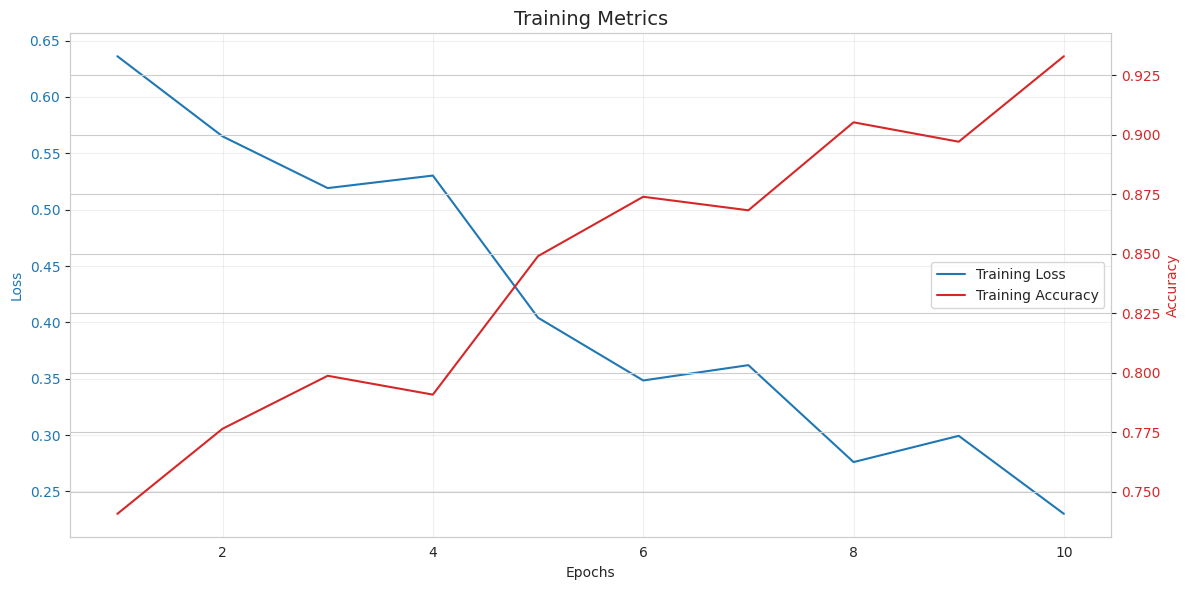
\includegraphics[width=0.45\linewidth]{training_metrics.png}

  Observations:
  \begin{itemize}
    \item Loss decreased steadily.
    \item Accuracy reached ~93.3% on training set at epoch 10.
  \end{itemize}
\end{frame}

% Classification Report
\begin{frame}{Test Set Evaluation Metrics}
  \vspace{-0.5em}
  {\small
    \begin{tabular}{lccc}
      Label            & Precision & Recall & F1-score     \\
      \hline
      Negative (0)     & 0.80      & 0.74   & 0.77         \\
      Positive (1)     & 0.78      & 0.83   & 0.80         \\
      Neutral (2)      & 0.52      & 0.52   & 0.52         \\
      \\[-0.8em]
      Overall Accuracy &           &        & {\bf 74.0\%} \\
    \end{tabular}}

  \vspace{1em}

  Key Insights:
  \begin{itemize}
    \item High precision/recall for Positive/Negative.
    \item Neutral class more ambiguous → lower performance.
  \end{itemize}
\end{frame}

% Confusion Matrix Image (Optional)
\begin{frame}{Confusion Matrix (Test Set)}
  \centering
  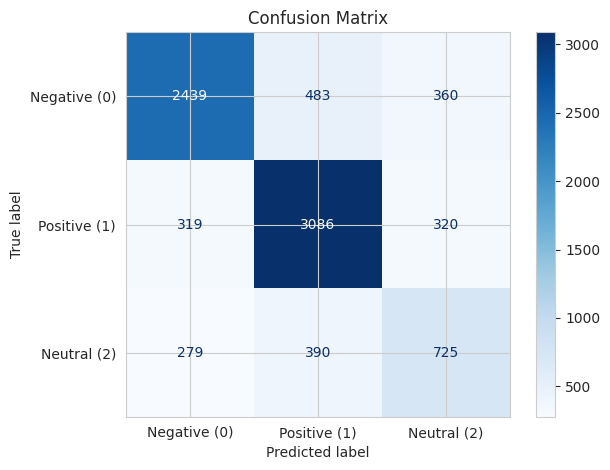
\includegraphics[width=0.45\linewidth]{confusion_matrix.png}

  Interpretation:
  Some overlap between Neutral and other classes → expected in real-world data.
\end{frame}

% Sample Predictions Table (Optional)
\begin{frame}{Sample Predictions on Unseen Data}
  \centering
  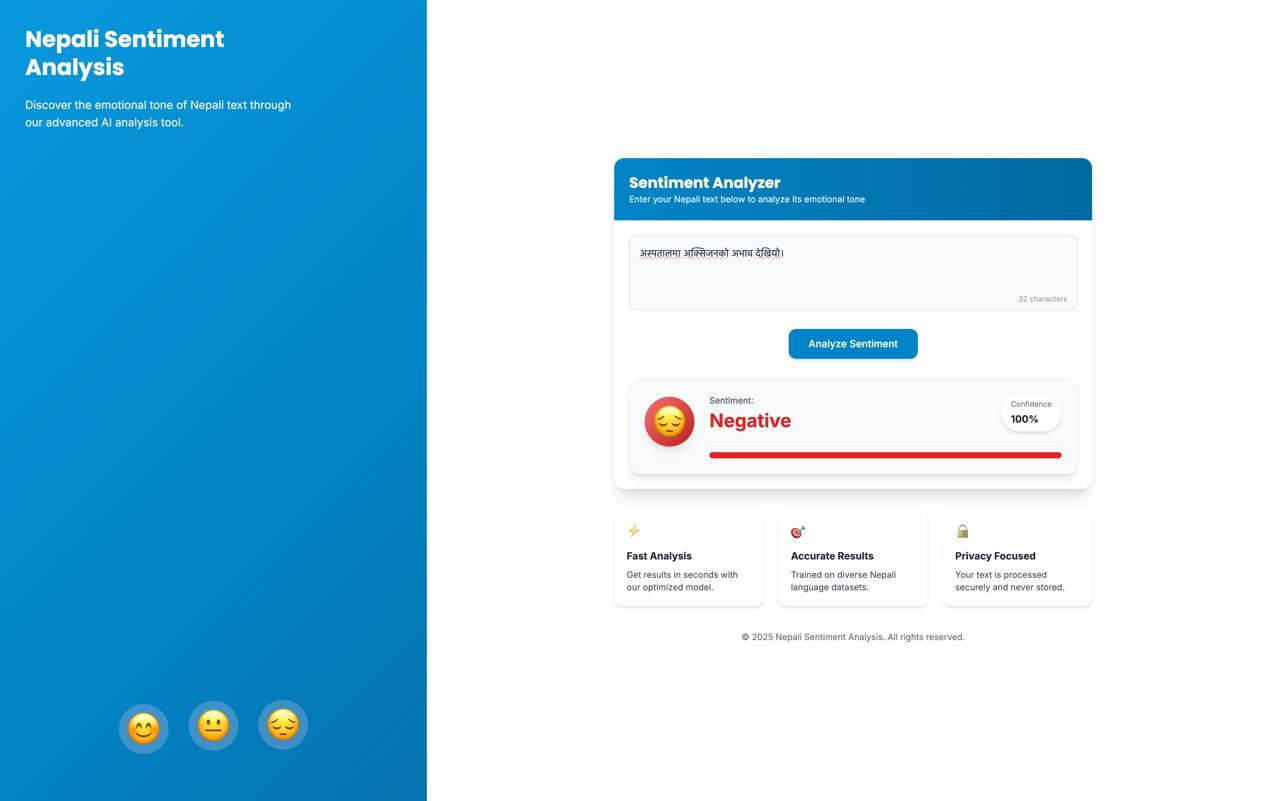
\includegraphics[width=0.75\linewidth]{visual.jpeg}
\end{frame}

% Conclusion slide
\section{Conclusion}
\begin{frame}{Conclusion and Future Work}
  Key Takeaways:
  \begin{itemize}
    \item Trained a sentiment classifier on Nepali-language text using XLM-Roberta.
    \item Achieved ~74% accuracy on test set.
    \item Strong performance on binary sentiment; neutral remains challenging.
  \end{itemize}

  Future Improvements:
  \begin{enumerate}
    \item Larger or augmented datasets.
    \item Additional validation set for tuning.
    \item Model deployment as an API/web service.
  \end{enumerate}
\end{frame}

% Thank You Slide
\section*{}
\begin{frame}{Thank You!}
  Questions or feedback?

  Project Resources:
  \vspace{-0.5em}

  {\footnotesize
  GitHub: {\texttt{\href{https://github.com/saileshbro/ai-proj}{github.com/saileshbro/ai-proj}}}}

  \vspace{-1em}

  We appreciate your time and attention!
\end{frame}

\end{document}
